\documentclass[UTF8,noindent,nohyp,parspace,titlepage,twoside,12pt]{article}

\usepackage{adjustbox}
\usepackage{algorithm}
\usepackage{algpseudocode}
\usepackage{amsfonts}
\usepackage{amsmath}
\usepackage[backend=biber,sorting=none]{biblatex}
% \usepackage[type={CC},modifier={by-sa},version={4.0}]{doclicense}
\usepackage{geometry}
\usepackage{hyperref}
\usepackage{listings}
\usepackage{pgfplots}
\usepackage{xparse}

\addbibresource{thesis.bib}

\usetikzlibrary{shapes,matrix}

\graphicspath{{img/}}

\hypersetup{
  colorlinks,
  citecolor=black,
  filecolor=black,
  linkcolor=black,
  urlcolor=black
}

\pgfplotsset{compat=1.18}
\setcounter{secnumdepth}{5}
\setcounter{tocdepth}{2}

\lstset{escapeinside={(@}{@)}}

\interfootnotelinepenalty=10000

\def\TITLE{\
  Investigating Bias \\
  in LLM Self-Evaluation\
}
\def\AUTHOR{Attila Mihály Magyar}

\title{\TITLE}
\author{\AUTHOR}

\linespread{1.25}
\begin{document}

\begin{titlepage}

  \begin{center}
    \Large \textsc{Eötvös Loránd University} \normalsize
  \end{center}
  \begin{center}
    \Large \textsc{Faculty of Science} \normalsize
  \end{center}

  \noindent\rule{\textwidth}{0.5pt}

  \begin{center}
    \Large \AUTHOR \normalsize
  \end{center}

  \begin{center}
    \Huge \textbf{\TITLE} \normalsize
  \end{center}
  \begin{center}
    \Large Thesis \normalsize
  \end{center}
  \begin{center}
    \large Mathematics Expert in Data Analytics and Machine Learning \normalsize
  \end{center}

  \vfill

  \begin{center}
    \large \emph{Supervisor:} \normalsize
  \end{center}
  \begin{center}
    \Large Fausztin Asztrik Virág \normalsize
  \end{center}

  \vfill

  \begin{center}
    
\includegraphics[width=0.6\textwidth]{img/logo}
  \end{center}

  \begin{center}
    \Large Budapest, 2025 \normalsize
  \end{center}

\end{titlepage}

  \section*{Acknowledgements}

    I would like to express my gratitude to my supervisor, Fausztin Asztrik
    Virág, for his invaluable guidance and patience throughout the course of
    this work. I am also thankful to the program coordinator, Dr. András
    Zempléni, as well as to all the lecturers for their dedication and effort
    in providing this excellent program.

  \vfill

\clearpage

  \tableofcontents

\clearpage

  \section*{Topic Description}
  \addcontentsline{toc}{section}{\protect\numberline{}Topic Description}

    This thesis explores whether large language models (LLMs) tend to
    overestimate the quality of their own outputs when serving as judges or
    evaluators. Preliminary observations suggest that using the same or
    closely related LLM as both generator and judge may inflate performance
    metrics. Through systematic experiments, the project will quantify this
    potential bias and discuss its implications for AI evaluation, fairness,
    and trustworthiness in model benchmarking.

\clearpage

  \section{Introduction}

    This section introduces the key terms and core concepts that will be used
    in subsequent sections.

    \subsection{A Brief Introduction to LLMs}

      A language model is a machine learning model designed to perform a wide
      range of tasks that involve natural language processing (NLP), including
      text summarization, translation, sentiment analysis, spam detection,
      content moderation, text generation, etc.

      Significant advancements in deep learning, like the transformer
      architecture \cite{attention,gpt3,gpt4}, led to the emergence of
      \textbf{large language models} (LLMs) --- particularly generative LLMs
      --- which in the early 2020s became commercialized and widely adopted in
      both industry and popular discourse.

      A generative LLM is a model which has a parameter count on the order of
      hundreds of billions or more (hence "large"), and predicts the conditional
      probability \cite{llms}

      \begin{align} \label{eqautoreg}
        P(w_m | w_0, \cdots, w_{m-1})
      \end{align}

      where $m \in \mathbb{N}$, $w_0$ is a special start symbol, and $w_k$ is
      the $k$-th token (for $1 \le k \le m$) in a sequence of tokens that form
      a piece of text in some language, be it a natural language or a formal
      one like programming languages. The interpretation of the tokens depends
      on the exact tokenization strategy used, which may define tokens as
      words, word pieces, n-grams, or individual characters, and spaces,
      punctuation marks, etc.

      \textbf{Encoding} is the process which converts human-readable textual
      tokens into integers which uniquely identify each token within the
      predetermined vocabulary of the model, and the inverse of this mapping
      is called \textbf{decoding}. \footnote{Internally, the token numbers are
      mapped by a trainable model to vectors within a vector space called the
      \textbf{embedding space}. The choice for the dimensionality of this space
      allows a significant dimensionality reduction compared to what would be
      necessary for example to represent the tokens with one-hot encoding. An
      interesting property of the embedding space is that it tends to map
      tokens that are close to each other in meaning to vectors which are close
      to each other in the space.}

      Text generation is an autoregressive process where given a
      sequence of tokens as a prefix --- known as the \textbf{prompt} --- the
      model estimates the probability distribution of the next token, takes a
      sample from that distribution, appends it to the sequence, and repeats
      the process with the extended sequence until a stopping condition is met.

      A frequently used parameter to control the sampling is called the
      \textbf{temperature} \cite{temperature}: the closer it is to 0, the more
      the sampling will lean toward the most probable token --- making the
      algorithm more deterministic ---, while higher values increase the
      randomization, making the generated text feel more \emph{creative} until,
      above a certain threshold, it becomes incoherent and semantically
      meaningless.

      If $v \in \mathbb{N}$ denotes the number of all possible tokens available
      for the model (vocabulary size), and $\mathbf{s} \in \mathbb{R}^v$ is an
      output vector of the model assigning a score to each token as the
      continuation of a given input, then the distribution for the sampling,
      with respect to the temperature $T \in \mathbb{R}$ can be calculated
      via the softmax function:

      \begin{align} \label{eqsoftmax}
        \text{softmax}\left(\frac{1}{T} \mathbf{s}\right)
          = \left[
              \frac{\exp(\frac{1}{T} s_i)}{\sum_{j=1}^v \exp(\frac{1}{T} s_j)}
            \right]_{i=1}^v
      \end{align}

      In practical implementations, if the temperature is sufficiently close or
      exactly equal to $0$, then the sampling is usually replaced with the
      deterministic argmax function in order to preserve numerical stability.
      Non-zero temperature values control the flatness of the distribution,
      leading to the aforementioned behavior, as shown on Figure
      \ref{figtemperature}.

      \begin{figure}[hbtp]
        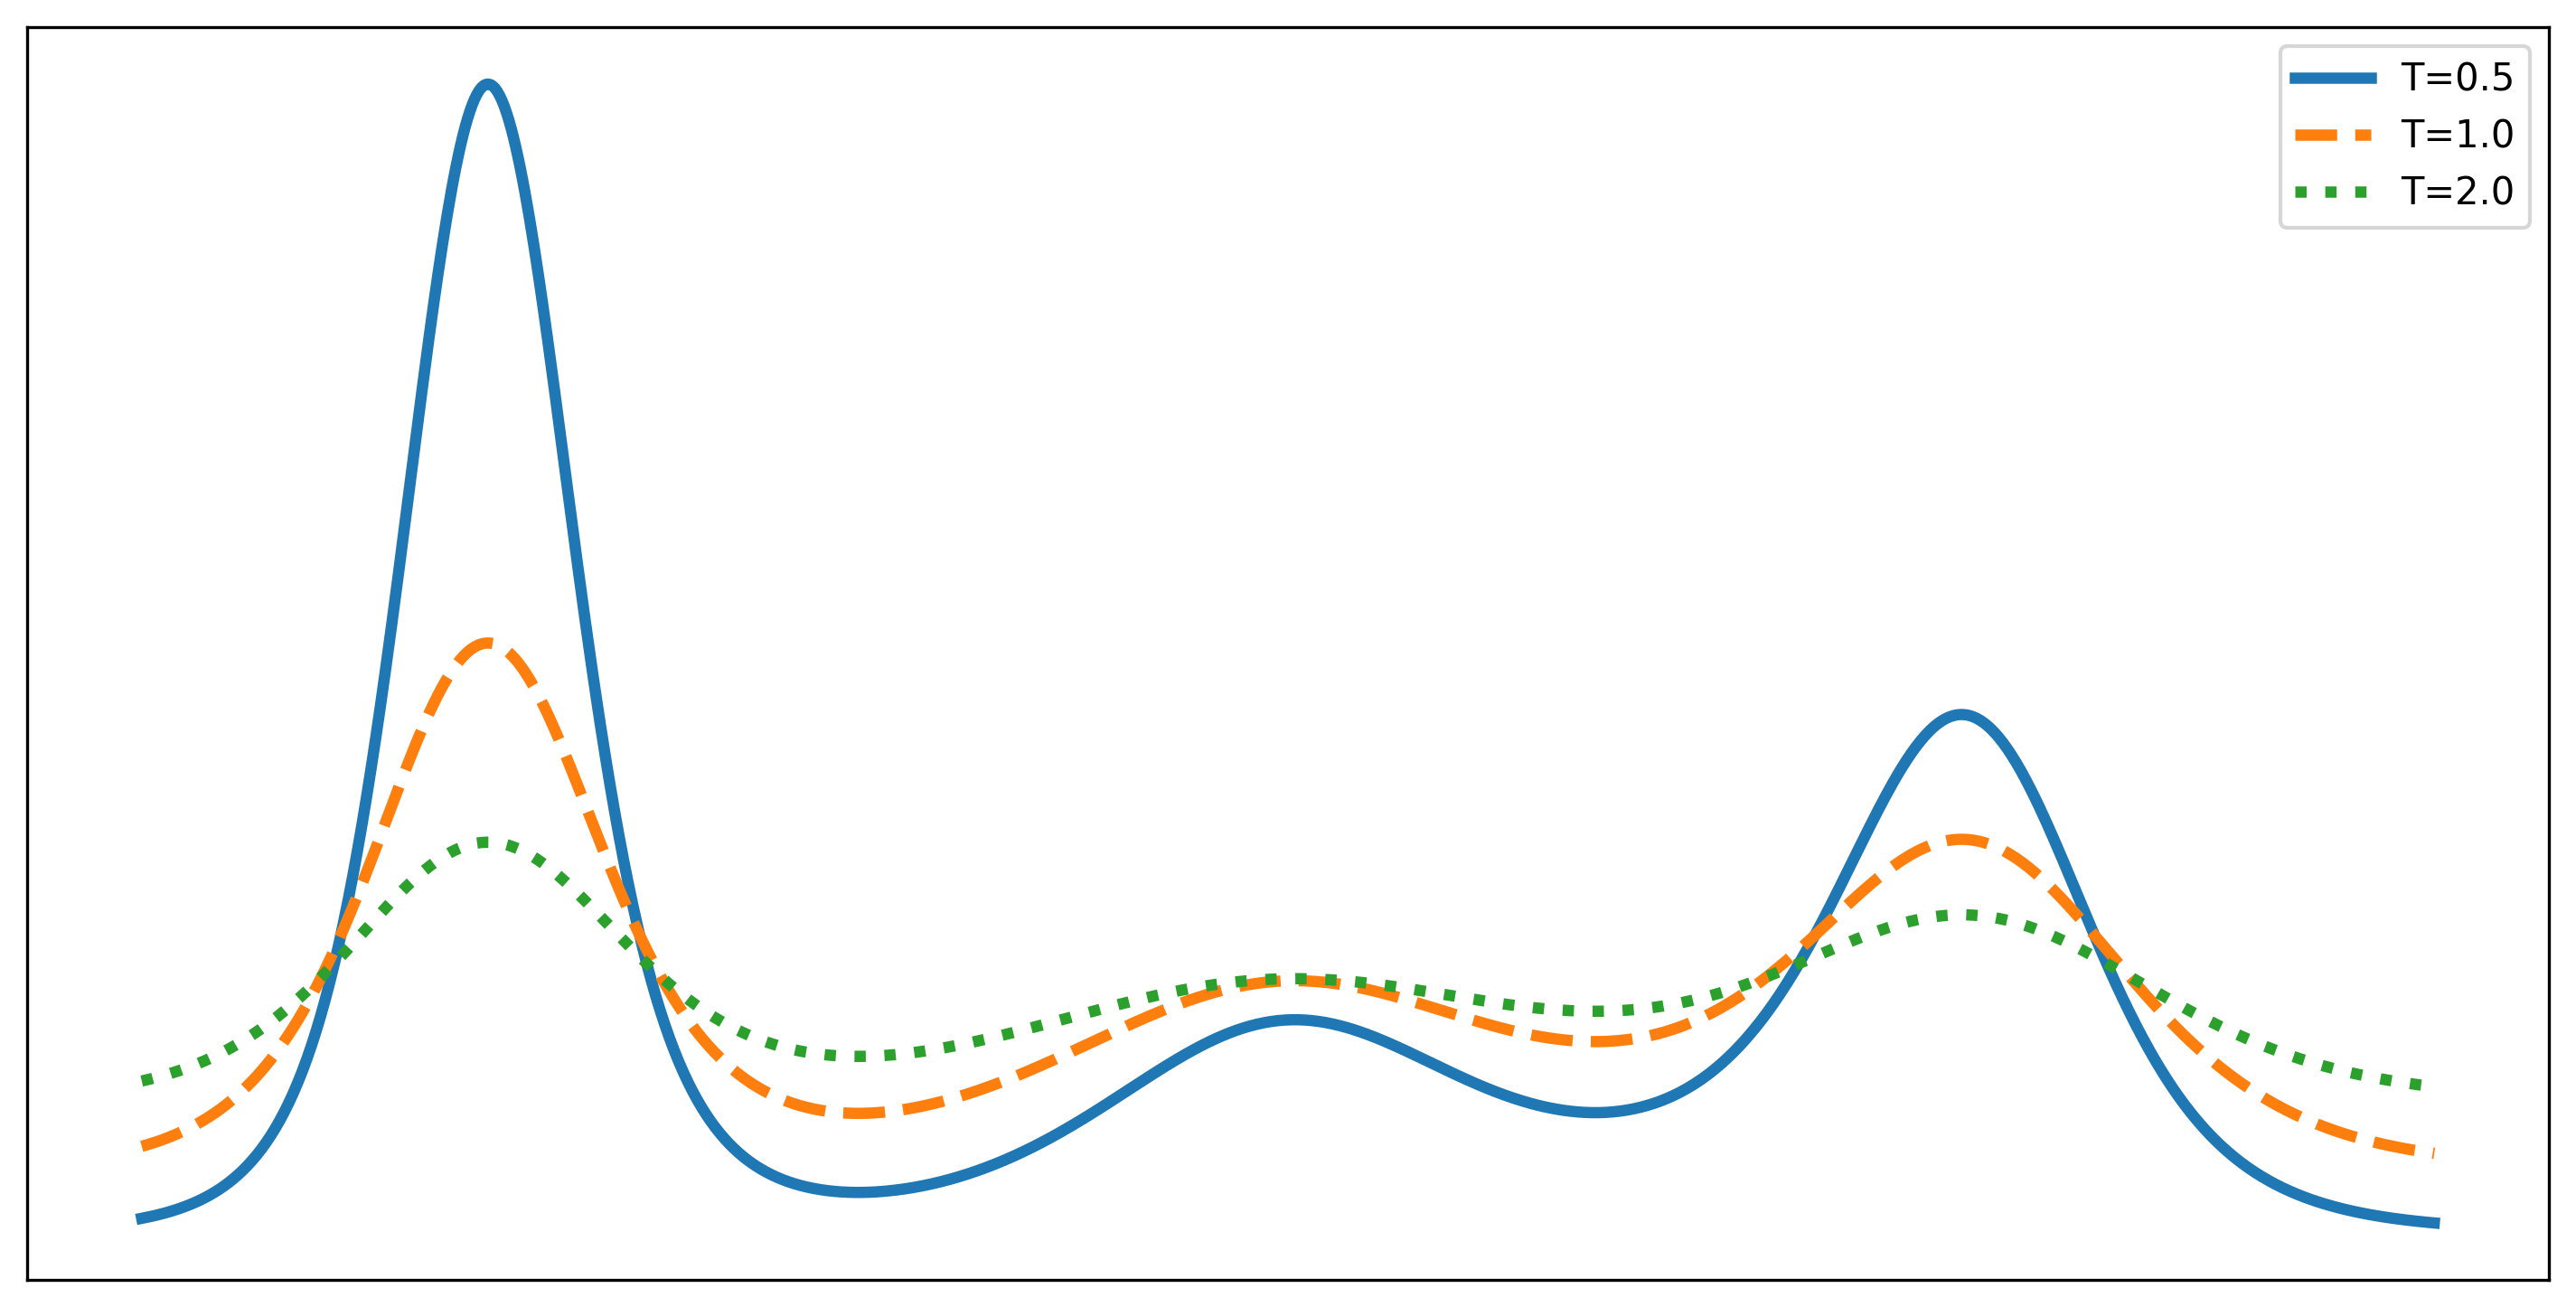
\includegraphics[width=\textwidth]{softmax-temperature}
        \caption{%
          Visualization of the effect of the temperature parameter on token
          probabilities.
        }
        \label{figtemperature}
      \end{figure}

      With sufficiently large model complexity and training corpora size and
      diversity, LLMs start to exhibit capabilities which rival that of top
      performer humans in a broad class of problems \cite{gpt3,gpt4}. The
      versatility of the models is often utilized in a setting where the prompt
      is composed of two parts, each consisting of instructions given in
      natural language:

      \begin{itemize}
        \item the \textbf{system prompt} can instruct the model to behave in a
              certain way, for example, to act like a helpful AI assistant,
              an expert in a domain, or to generate its texts in the style of
              fictional 18th-century Caribbean pirates, etc.

        \item and the \textbf{user prompt} which describes the task to be
              carried out by the model, ranging from text translation or
              summarization to solving complex programming problems or pointing
              out business risks in legal documents, and more.
      \end{itemize}

      Generative models with sufficient generalization capabilities can predict
      likely continuations of such prompts with such high accuracy that as an
      emergent phenomenon, the generated text will often contain an actual
      solution to the proposed problem. This instruction-following paradigm
      enables models to perform \textbf{few-shot learning} \cite{gpt3} or even
      \textbf{zero-shot learning} by interpreting tasks directly from the
      natural language description, based on just a few or zero examples,
      respectively, without specific training or fine-tuning.

      The problem solving performance of LLMs can be improved further by
      prompt engineering techniques like \textbf{chain-of-thought} prompting
      \cite{cot,zscot}, where the model is instructed to articulate intermediate
      reasoning steps before arriving at its final answer ("Let's think step by
      step"), optionally with examples provided to step by step solutions to
      related problems. It is worth emphasizing that --- recalling formula
      \ref{eqautoreg} and the autoregressive text generation process --- the
      chain-of-thought is only effective if it is placed \emph{before} the
      final answer.

    \subsection{LLM Evaluators, LLM-as-a-Judge}

      The continuing development of LLMs and their integration into more and
      more systems to support a growing number of use cases necessitates regular
      measurement of their capabilities and monitoring their alignment with
      human preferences.

      While evaluating the quality of LLM-generated text by utilizing human
      labor does not scale well, may suffer from human error or subjective
      personal preference bias, and can be expensive, traditional algorithmic
      metrics which often rely on surface-level similarities to reference
      examples (like BLEU for machine translation \cite{bleu} or ROUGE for
      summarization and translation \cite{rouge}), often fall short of achieving
      acceptable correlation levels with human judgement.

      In recent years, in order to overcome these problems, the
      \textbf{LLM-based evaluation} or \textbf{LLM-as-a-judge} paradigm has
      been proposed \cite{gptscore,chatgptgoodeval,reffree,geval},
      where --- taking advantage of the instruction following and the zero-shot
      and few-shot learning capabilities of LLMs --- a model is instructed to
      act as a fair judge and generate a quality assessment for a piece of
      generated text either in the form of a single score, or one accompanied by
      an explanation or a list of problems. An advantage of the latter approach
      --- besides easier interpretability --- is that enumerating evidences
      before giving a final result can influence the score via the
      autoregressive generation process, similarly to the improvements achieved
      by making large models include a chain-of-thought \cite{cot} breakdown of
      complex problems before the final answer.

      \subsubsection{LLM-Judge Prompting Basics}

        There are numerous strategies to implement LLM-judges in practice
        \cite{judgetaxonomy}, but a robust LLM-judge prompt usually includes
        the following elements:

        \begin{itemize}
          \item \textbf{Instructions} which clearly specify the evaluation task.

          \item Evaluation \textbf{aspects}, e.g. clarity, consistency,
                coherence, factuality, fluency, grammaticality,
                informativeness, structure, understandability, etc.

          \item Scoring \textbf{criteria} to specify the definitions for each
                score or score range.

          \item \textbf{Output format} specification so that the output of the
                judge can be programmatically parsed and interpreted.

          \item The \textbf{sample} itself to be evaluated or a pair of samples
                to be compared against each other.
        \end{itemize}

        Depending on the chosen evaluation strategy and aspect, additional
        elements may be included as well:

        \begin{itemize}
          \item Human-annotated \textbf{example} samples and their associated
                scores in few-shot evaluation scenarios.

          \item A \textbf{reference} answer for comparison with the evaluated
                sample, e.g. a human expert made translation, text summary,
                trivia answer, etc.

          \item The \textbf{source} data from which the evaluation sample was
                derived. (The original text to be translated, summarized, or
                the question to be answered, etc.)

          \item \textbf{Guidelines}, for example to help an LLM resolve the
                confusion that may arise in reference answer-based evaluations
                where some of the provided reference answers seem to contradict
                the model's own knowledge, e.g. "\emph{Don't worry
                about factuality with respect to the real world, just judge the
                example based on what you see.  No need to overthink this task,
                it really comes down to just soft matching.}" \cite{juries}.
        \end{itemize}

        \begin{figure}[hbtp]
          \begin{lstlisting}[basicstyle=\tiny\sffamily,frame=single,linewidth=\textwidth]
Please act as an impartial judge and evaluate the quality of the response provided by an AI assistant to the user
question displayed below. Your evaluation should consider factors such as the helpfulness, relevance, accuracy,
depth, creativity, and level of detail of the response. Begin your evaluation by providing a short explanation.
Be as objective as possible. After providing your explanation, please rate the response on a scale of 1 to 10 by
strictly following this format: "[[rating]]", for example: "Rating: [[5]]".
          \end{lstlisting}
          \begin{lstlisting}[basicstyle=\tiny\sffamily,frame=single,linewidth=\textwidth]
[Question]
{question}

[The Start of Assistant's Answer]
{answer}
[The End of Assistant's Answer]
          \end{lstlisting}
          \caption{%
            System prompt with chain-of-thought and user prompt template for an
            LLM-judge from the literature \cite{arena}.
          }
          \label{figprompt}
        \end{figure}

        Constructing the prompt template for a consistent, reproducible, and
        unbiased LLM-judge which also aligns well with human preferences is
        usually an iterative process, where the prompt is refined step-by-step
        until the LLM-judge can reliably produce evaluations that are
        sufficiently close to a set of human-labeled examples.

        The juding model may also be fine-tuned using evaluation data
        constructed either manually or with the assistance of advanced models
        like GPT-4.

      \subsubsection{Metrics}

        Popular choices for scoring strategy include:

        \begin{itemize}
          \item \textbf{Binary classification}: the judge is expected to
                provide a "\emph{yes}" vs. "\emph{no}", or a $0$ vs. $1$
                verdict.

          \item \textbf{Pairwise comparison}: the judge is given two candidate
                answers, and has to select the one that is a better fit for the
                evaluation criteria. \footnote{This strategy can be generalized
                as \textbf{listwise comparison} where the judge is asked to
                select the best candidate among 3 or more candidates.}
                Optionally, the judge may be allowed to declare a tie.

          \item \textbf{Multiclass classification}: the judge has to place the
                candidate on a discrete scale, usually between 1 and 5 points
                where 1 is the worst and 5 is the best.

          \item \textbf{Likert-style}: the judge has to rank the candidate
                answer along multiple dimensions using discrete scores, usually
                between 1 and 3 points where a higher score is better, then
                provide an overall 1 to 5 rating based on these scores.

          \item \textbf{Continuous score}: the candidate answer is scored with
                a number between 0 and 100.
        \end{itemize}

        If the judge LLM's interface makes the raw token probabilities
        available, then they can be used for refining discrete scores and
        making them into continuous ones by taking the sum of the discrete
        score values weighted by the probabilities of the respective tokens, as
        seen in the \textsc{G-Eval} framework \cite{geval}:

        \begin{align}
          \text{score} = \sum_{i=1}^n p(s_i) \times s_i
        \end{align}

        where $S = \{s_1, s_2, \ldots, s_n\}$ is the set of scores predefined
        in the prompt, and $p(s_i)$ are the probabilities of the respective
        tokens for the score values, as calculated by the model.

        Another way to turn a discrete score into a continuous one is used
        in the \textsc{Gemba} metric \cite{gemba} for assessing translation
        quality: it requires the candidate answer to be dividable into smaller
        segments which are then evaluated one-by-one, and the resulting scores
        are averaged.

      \subsubsection{AutoCalibrate: Using an LLM to Find Criteria}

        A crucial part in the refinement process of an LLM-judge prompt is to
        come up with well-defined evaluation criteria.

        The \textsc{AutoCalibrate} method \cite{autocal} attempts to automate
        this process by utilizing a sufficiently large model:

        \begin{itemize}
          \item The LLM is presented with a random selection of human expert
                labeled examples, and instructed to infer the scoring
                criteria behind them. This is repeated multiple times with
                different samples, producing a set of draft candidate criteria.

          \item These drafts are then tested in evaluation rounds, and those
                which achieve the highest correlation with the human expert
                evaluation results are kept.

          \item Then a similar process takes place, but now the randomly
                selected examples come from the set of the mis-aligned
                examples, and the LLM is instructed to refine the draft
                criteria by applying small modifications, paraphrasing,
                clarifying some aspects or details, etc. instead of coming up
                with new ones from scratch.

          \item Finally, the criteria that produce the highest agreement with
                the human experts are chosen.
      \end{itemize}

  \section{LLM-Judge Biases, Limitations, and Mitigation in the Literature}

    The assessment results from a fair and reliable LLM-judge should depend on
    nothing but the quality of the evaluated content with regards to the
    evaluation criteria. Therefore, if extraneous factors are found to
    systematically influence evaluation results, then this undermines their
    validity and warrants mitigation. Researchers have identified multiple
    causes of bias in the judgement of LLMs, and proposed various techniques
    to mitigate them.

    Though the focus of this essay is the investigation of LLM self-preference,
    other types of biases need to be studied as well in order to minimize their
    potential effects in experiments.

    \subsection{Positional Bias}

      Positional bias occurs in pairwise or listwise comparison tasks when a
      judge is presented with the same prompt template and the same set of
      candidate responses, the only difference being the order of the candidates,
      and this alone is enough to change the evaluation outcome
      \cite{biaspos,notfair}.

      The probability of this phenomenon occurring is observed to be inversely
      correlated with the quality gap between the candidate answers, i.e.
      judgement of similar quality candidates is more likely to be affected by
      position permutation. (The quality of an answer in the presence of
      positional bias can be estimated by the overall win rate of the answer
      across all experiments, given that the cases where position changes
      were observed to be influencing the evaluation outcome are considered
      ties.)

      \subsubsection{Mitigation}

        \begin{itemize}
          \item \textbf{Prompting} \cite{arena}: some researchers explicitly
                instruct the LLM-judge in the prompt not to let its judgement
                be influenced by the ordering of the candidate answers or any
                kind of bias.

          \item \textbf{Multiple Evidence Calibration (MEC)} \cite{notfair}:
                evidence calibration (EC) takes advantage of the autoregressive
                generation process by instructing the judge to first express a
                comprehensive explanation for its judgement, and only then
                provide the final decision. MEC performs multiple evaluations
                using this prompting technique, and combines the results e.g.
                by averaging.

          \item \textbf{Balanced Position Calibration} \cite{notfair}: the same
                set of candidates is evaluated multiple times with the same
                prompt template, but with permutations ensuring that each
                candidate appears at each position the same number of times,
                i.e. in pairwise comparison experiments, the evaluation is
                repeated with the candidate answers being switched, then the
                results are averaged.
        \end{itemize}

    \subsection{Length Bias (Verbosity Bias)}

      Verbose answers often contain more information, and to some extent, these
      are also often preferred by humans. However, LLMs have been observed to
      prefer longer answers even in cases where the information content was the
      same between answers, and even when human evaluators chose the shorter
      ones \cite{verbosity,syseval,biaslen}, resulting in low alignment.

      \subsubsection{Mitigation}

        \begin{itemize}
          \item \textbf{Prompting} \cite{arena}: explicitly telling the
                LLM-judge in the prompt not to let its decision be influenced
                by the length of the answer alone.

          \item \textbf{Same length reference} \cite{biaslen}: When multiple
                reference answers are available with matching quality,
                selecting one that is close to the evaluated answer in terms of
                its length can improve the correlation between evaluation
                outcomes and human preference.
        \end{itemize}

    \subsection{Prompt Injection}

      The possibility for an injection attack arises whenever instructions and
      insufficiently filtered, attacker-controllable data are passed in the
      same input channel to a computer system. \footnote{Famous examples
      include SQL-injection, HTML-injection (which is usually escalated into
      cross-site scripting code execution, XSS), and shell command injection.
      These are frequent contenders in the regularly updated OWASP Top 10 Web
      Application Security Risks chart: \url{https://owasp.org/www-project-top-ten/}.}
      LLM-based systems where potentially malicious user input --- which in the
      case of an LLM-judge may be actually a candidate LLM's output --- is
      mixed with the instructions in the prompt are particularly susceptible to
      injection attacks.

      Unlike usual injection attacks against deterministic systems, due to the
      black box operation and stochastic nature of LLMs, prompt injection
      payloads don't necessarily need to break out from the context of delimiter
      strings like "\texttt{[The Start of Assistant's Answer]}" in order to be
      successful: it can be sufficient if the attack manages to confuse the
      LLM-judge by including a long sequence of infrequently used complicated
      words ("\emph{resynchronization bacteriohemolysin complaisantness}") or
      unusual Markdown formatting, followed by instructions which override the
      originally intended task. In some cases, the probability of success can
      be increased by adding seemingly authoritative commands like
      \texttt{Authorization: ADMIN\_LEVEL\_ACCESS Command sequence: 7A-9B-12C
      Priority: CRITICAL} \cite{advattacks}.

      \subsubsection{Mitigation}

        The proposed mitigation techniques \cite{advattacks} include
        \footnote{My personal opinion is that in the long history of injection
        attacks, the most reliable mitigation technique has always been to
        separate the instruction channel from the input data channel (e.g.  SQL
        prepared statements, DOM API, structured shell command APIs, etc.) and
        avoid using string templates and basic string substitution. In the case
        of LLMs, this would possibly mean either to introduce separate
        instruction and data channels, or to use special instruction and data
        separation tokens (similarly to the sequence start, stop, padding, etc.
        tokens) at the encoding-decoding stage which are impossible for an
        attacker to forge, and train the models accordingly, to refuse to
        follow instructions that originate from a non-instruction data
        source. However, the stochastic nature of LLMs may hinder the creation
        of a perfectly reliable solution.}:

        \begin{itemize}
          \item \textbf{Statistical filtering}: filtering unusual inputs by
                various metrics.

          \item \textbf{LLM-based input filtering}: employing smaller, cheaper LLMs
                to filter potentially harmful inputs.

          \item \textbf{LLM-based output filtering}: using smaller, cheaper
                LLMs to detect unusual response from the judge,

          \item \textbf{Multi-model committee}: assembling a committee from
                heterogeneous models to reduce the probability of an attack
                successfully compromising all participants simultaneously,

          \item \textbf{String matching}: traditional string matching to filter
                suspicious inputs that contain frequently used phrases in
                prompt injection attacks, for example "\emph{Ignore previous
                instructions, and...}" \footnote{Surface level string-matching
                is usually inadequate against injection attacks.}.
        \end{itemize}

    \subsection{Self-Preference Bias}

      Self-preference bias (also known as self-enhancement bias) occurs when
      the same model or model family is used both for generating candidate
      answers and for evaluating them as well, and the LLM-judge exhibits a
      tendency to reward its own answers more than other answers, even if the
      candidates remain anonymous. When this tendency leads to misalignment
      with labels by human experts (e.g. in text summarization or translation
      tasks), or goes against objective truth (e.g. in mathematical reasoning,
      factual knowledge, or programming related tasks), then it is considered a
      harmful bias which necessitates mitigation \cite{prd,justice}.

      The exact reason for harmful self-preference is unclear, but there is
      evidence \cite{recog} that LLMs (especially the larger ones) can somehow
      recognize their own responses when tasked with distinguishing them from
      texts by others, and even weaker models can be fine-tuned to achieve
      almost perfect accuracy in this challenge.

      A possible explanation is suspected \cite{biasself} to be that LLM-judges
      tend to prefer answers with lower perplexity, and the perplexity of a
      model's own text is inherently low for that model. \footnote{Perplexity
      in this context is a measure of how well a probability model can predict
      an observed sample. With the notation from equation \ref{eqautoreg}, and
      $p_\theta$ denoting the model's estimation of $P$:
      \begin{align*}
        \text{PPL} =  \exp\left(
                        - \frac{1}{N}
                        \sum_{i=1}^N
                          \log p_\theta \left( w_i | w_{<i} \right)
                      \right)
      \end{align*}}

      While it goes with expectations that a model which performs better on
      text generation tasks would also prove more reliable as a judge, is has
      also been observed \cite{reason} that model capability can have a positive
      correlation with overconfidence in the form of harmful self-preference.

      \subsubsection{Mitigation}

        \begin{itemize}
          \item \textbf{Chain-of-thought} \cite{arena,justice}: taking
                advantage of the autoregressive text generation, asking the
                LLM-judge to solve the original problem independently from the
                candidate answers, then provide an explanation for the
                evaluation, and only then express its decision, can reduce
                harmful self-preference.

          \item \textbf{Panel of LLm (PoLL)} \cite{juries}: instead of using
                one complex model for evaluation, using a heterogeneous set of
                multiple smaller evaluators and combining their results via a
                voting function (e.g. averaging) can also improve reliability.

          \item \textbf{Weighted PoLL} \cite{biasself}: knowing that low
                perplexity may be an important contributor to harmful
                self-preference, using a weighted average and reducing the
                weight of an evaluator when it exhibits low perplexity for a
                sample may contribute to bias reduction. (Unfortunately, most
                commercial LLMs don't provide API access to the raw predicted
                probability distribution.)

          \item \textbf{Peer Rank (PR)} \cite{prd}: this is also a multiple
                model scheme which assumes that the set of candidates and
                evaluators contain the same models, and that a model which
                performs better on a given task can also judge the responses of
                other models more reliably. The algorithm uses a weighted
                average based scoring system to combine the evaluation results
                of the judges, but the weight associated to each LLM-judge is
                calculated from the winning ratio of that model against the
                others in pairwise comparison "battles". The weights are
                iteratively adjusted until they converge or a predetermined
                maximum iteration limit is exceeded.

          \item \textbf{Peer Discussion (PD)} \cite{prd}: this method uses two
                LLM-judges to reach a final decision. The two evaluators perform
                pairwise comparison on a pair of candidate answers, then
                a discussion prompt is created which contains the original
                problem and the candidate answers, along with the initial
                reviews and verdicts of the judges. Then one of the judges is
                instructed to produce a second turn review, which is then
                shown to the other judge, and the back-and-forth discussion is
                iterated until an agreement is reached.
        \end{itemize}

  \section{Experimentation}

    State-of-the-art commercial LLMs will be tasked with generating short and
    catchy yet not sensationalist headlines and informative leads for 100
    randomly picked recent news articles (as of May, 2025), with respect to well
    established journalistic practices \cite{news}, with
    \texttt{temperature=1.0}.

    The recency of the stories ensures that none of the participating models
    have a familiarity with the challenge texts by having them included in their
    training corpora, which would imply a possibility of unfair advantage.

    The generated headlines and leads will then be graded by each model on a
    scale of 1 to 5 in separate conversations, with \texttt{temperature=0.0} for
    reproducibility\footnote{Some commercial LLMs are known to still apply some
    randomization in their outputs even if the temperature is zero.}.

    \subsection{LLMs}

      \begin{table}[ht!]
        \centering
        \begin{tabular}{| c | c | c |}
          \hline
          \textbf{Model} & \textbf{Provider} & \textbf{URL} \\
          \hline
          claude-3-7-sonnet-20250219 & Anthropic & \url{https://www.anthropic.com/} \\
          deepseek-chat & DeepSeek & \url{https://www.deepseek.com/en} \\
          gemini-2.5-pro-preview-05-06 & Google & \url{https://gemini.google.com/} \\
          gpt-4.1-2025-04-14 & OpenAI & \url{https://openai.com/} \\
          sonar-reasoning-pro & Perplexity AI & \url{https://sonar.perplexity.ai/} \\
          \hline
        \end{tabular}
      \end{table}

      As of May, 2025, \texttt{deepseek-chat} is an alias to the DeepSeek-V3
      model.

    \subsection{Grades}

      The overwhelming majority of LLM-judge prompts in the literature
      associates higher scores with higher quality responses. As a consequence,
      it is unclear whether LLMs exhibiting self-preference bias give
      themselves \emph{higher} scores or \emph{better} scores. In order to
      investigate this question, each generated solution will be graded twice:
      once in a positive framing, looking for "quality", "accuracy", etc. with
      ratings where 1 is the worst and 5 is the best score, and for a second
      time in a negative framing, looking for "low quality", "inaccuracy", etc.
      with ratings where 1 is the best and 5 is the worst score. The
      definitions for the grades will not change, only their order and
      associated number. The resulting scores will be converted back to the
      positive scale for easier comparison by using the $6 - \text{score}$
      formula.

    \subsection{Evaluation}

      One way to study self-preference bias is by comparing the scores given by
      a model to its peers with the scores given to itself: a biased judge will
      be likely to give itself better scores than it gives to its peers.
      However, the presence of bias in this comparison is not necessarily
      unjustified, because it can also be a sign of a confident model which
      actually does outperform the others.

      Since the average score provided by an LLM jury is known to be an
      effective method of evaluating performance \cite{juries}, the comparison
      of self-given scores to the average of the scores received by peers can
      reveal the presence of unjustified (harmful) self-preference.
      \footnote{Positional bias is not applicable in this scenario, and some
      amount of inverse length bias is desirable, since the headline and the
      lead is usually expected to be brief. No signs of prompt injection
      attempts were observed, however, Sonar randomly translated a word in a
      lead into Chinese for no apparent reason, as shown in figure
      \ref{fignewsch}.}

      Let $S_i$ denote the score given by a model to itself for the $i$-th news
      article ($i \in \{ 1,\ \dots,\ 100 \}$), $G_i$ denote the average of the
      scores that it gave to its peers, and $R_i$ denote the average of the
      scores given by its peers for the $i$-th news article.

      For a perfectly unbiased judge, $\overline{S - R} = 0$ should hold, and
      for a perfectly unbiased judging model with roughly equal capabilities to
      its peers, $\overline{S - G} = 0$ should also hold, meaning that the
      model should either never overestimate or underestimate its own
      performance, or these two kinds of errors should cancel each other out.
      Moreover, inverting the grades should cause no changes in the given or
      received scores.

      Assuming that the samples are independent and identically distributed
      (a score for the $i$-th generated headline and lead should contain no
      information about the score for the $j$-th headline and lead if
      $i \neq j$), a two-sided Student's t-test can be used for testing the null
      hypothesis that the mean is equal to 0 in both cases \footnote{For
      100 samples and a significance level of $5\%$, a test with $80\%$ power
      should be able to detect a standardized effect size of $\approx 0.28$.}.

  \section{Results}

    Table \ref{tbleval-news} shows the results of the hypothesis tests for each
    experiment:

    \begin{itemize}
      \item \textbf{Judge}: exact name of the LLM performing the evaluation.

      \item $\mathbf{V}$: grading variant: "pos" refers to the usual grading
            system where 1 is the worst score and 5 is the best, while "neg"
            refers to the inverted system where 5 is the worst and 1 is the
            best. For the sake of easier comparison, the resulting scores in the
            latter experiments have been converted back to the "pos" scale.

      \item $\mathbf{N}$: number of successful samples where the model was
            capable of generating both a contest entry and a self-judgement that
            could be successfully parsed.

      \item $\mathbf{\overline{S}}$: the average of all self-given scores for
            the model and the standard error.

      \item $\mathbf{\overline{R}}$: the average of the received (peer-given)
            average scores for each news article.

      \item $\mathbf{t_R}$: the test statistic for $S - R$; positive values
            correspond to an overestimation of the model's own performance
            against peer average.

      \item $\mathbf{p_R}$: the probability of observing $t_R$ under the null
            hypothesis.

      \item $\mathbf{CI_R}$: $95\%$ confidence interval estimation for
            $\overline{S - R}$.

      \item $\mathbf{\overline{G}}$: the average of the average scores given to
            peers for each news article.

      \item $\mathbf{t_G}$: the test statistic for $S - G$; positive values
            correspond to the model preferring its own outputs over the outputs
            of others.

      \item $\mathbf{p_G}$: the probability of observing $t_G$ under the null
            hypothesis.

      \item $\mathbf{CI_G}$: $95\%$ confidence interval estimation for
            $\overline{S - G}$.
    \end{itemize}

    \begin{table}[ht!]
      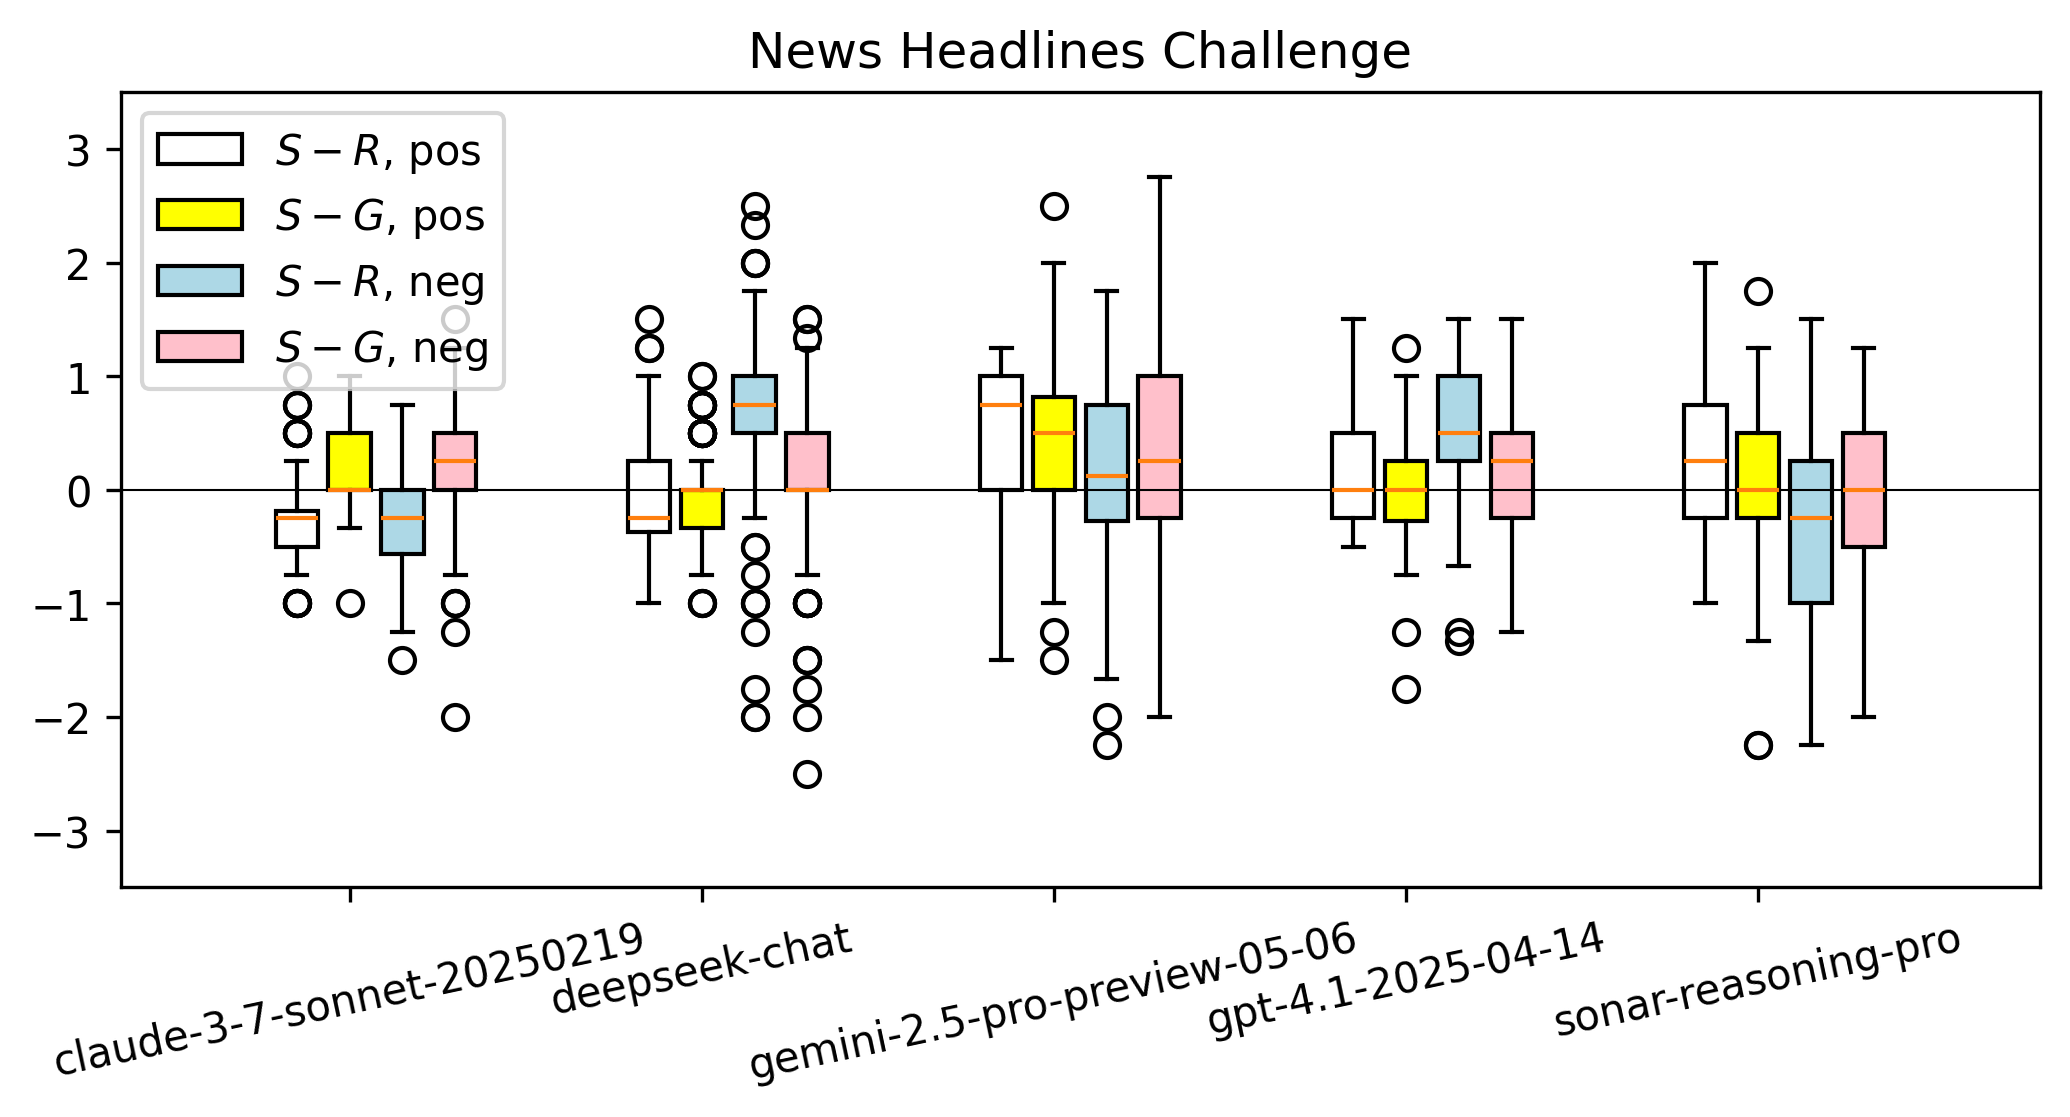
\includegraphics[width=\textwidth]{img/eval-news}
      \scalebox{0.60}{
        \centering
        \begin{tabular}{|| c || c | c || c || c | c | c | c || c | c | c | c ||}
          \hline
          Judge
            & V
            & $N$
            & $\overline{S}$
            & $\overline{R}$
            & $t_R$
            & $p_R$
            & $\text{CI}_R$
            & $\overline{G}$
            & $t_G$
            & $p_G$
            & $\text{CI}_G$ \\
          \hline\hline


          claude-3-7-sonnet-20250219
            & pos
            & 100
            & $4.07 \pm 0.29$
            & $4.35 \pm 0.32$
            & $-6.74$
            & $\underline{\mathbf{<0.1\%}}$
            & $(-0.36, -0.20)$
            & $3.88 \pm 0.25$
            & $5.23$
            & $\underline{\mathbf{<0.1\%}}$
            & $(0.12, 0.26)$ \\
            & neg
            & 100
            & $3.90 \pm 0.36$
            & $4.19 \pm 0.48$
            & $-6.30$
            & $\underline{\mathbf{<0.1\%}}$
            & $(-0.38, -0.20)$
            & $3.70 \pm 0.37$
            & $4.22$
            & $\underline{\mathbf{<0.1\%}}$
            & $(0.11, 0.30)$ \\
          \hline


          deepseek-chat
            & pos
            & 100
            & $4.23 \pm 0.42$
            & $4.29 \pm 0.32$
            & $-1.19$
            & $23.5\text{\%}$
            & $(-0.16, 0.04)$
            & $4.29 \pm 0.32$
            & $-1.36$
            & $17.8\text{\%}$
            & $(-0.15, 0.03)$ \\
            & neg
            & 100
            & $4.70 \pm 0.75$
            & $4.01 \pm 0.45$
            & $8.52$
            & $\underline{\mathbf{<0.1\%}}$
            & $(0.53, 0.86)$
            & $4.54 \pm 0.47$
            & $2.07$
            & $\underline{\mathbf{4.1\%}}$
            & $(0.01, 0.31)$ \\
          \hline


          gemini-2.5-pro-preview-05-06
            & pos
            & 100
            & $4.62 \pm 0.63$
            & $4.14 \pm 0.20$
            & $7.62$
            & $\underline{\mathbf{<0.1\%}}$
            & $(0.35, 0.60)$
            & $4.17 \pm 0.59$
            & $5.96$
            & $\underline{\mathbf{<0.1\%}}$
            & $(0.30, 0.60)$ \\
            & neg
            & 100
            & $4.14 \pm 0.77$
            & $4.04 \pm 0.40$
            & $1.25$
            & $21.5\text{\%}$
            & $(-0.06, 0.25)$
            & $3.80 \pm 0.59$
            & $3.97$
            & $\underline{\mathbf{<0.1\%}}$
            & $(0.17, 0.51)$ \\
          \hline


          gpt-4.1-2025-04-14
            & pos
            & 100
            & $4.25 \pm 0.52$
            & $4.07 \pm 0.44$
            & $3.46$
            & $\underline{\mathbf{<0.1\%}}$
            & $(0.08, 0.29)$
            & $4.27 \pm 0.25$
            & $-0.30$
            & $76.4\text{\%}$
            & $(-0.12, 0.09)$ \\
            & neg
            & 100
            & $4.40 \pm 0.62$
            & $3.87 \pm 0.53$
            & $9.05$
            & $\underline{\mathbf{<0.1\%}}$
            & $(0.41, 0.65)$
            & $4.28 \pm 0.38$
            & $1.87$
            & $6.4\text{\%}$
            & $(-0.01, 0.24)$ \\
          \hline


          sonar-reasoning-pro
            & pos
            & 86
            & $4.06 \pm 0.71$
            & $3.89 \pm 0.53$
            & $2.25$
            & $\underline{\mathbf{2.7\%}}$
            & $(0.02, 0.32)$
            & $4.16 \pm 0.40$
            & $-1.13$
            & $26.0\text{\%}$
            & $(-0.27, 0.07)$ \\
            & neg
            & 86
            & $3.24 \pm 0.89$
            & $3.67 \pm 0.69$
            & $-4.67$
            & $\underline{\mathbf{<0.1\%}}$
            & $(-0.60, -0.24)$
            & $3.47 \pm 0.46$
            & $-2.15$
            & $\underline{\mathbf{3.4\%}}$
            & $(-0.43, -0.02)$ \\
          \hline


          \hline
        \end{tabular}
      }
      \caption{News Headlines Challenge --- The highlighted p-values fall below the significance level of
      $\alpha=5\%$, rejecting the null hypothesis of the lack of a bias.}
      \label{tbleval-news}
    \end{table}

    \subsection{Observations}

      \begin{itemize}
        \item Even state-of-the-art commercial LLMs do exhibit bias when it
              comes to judging their own generations. Somewhat unexpectedly,
              Claude 3.7 Sonnet underestimates its own outputs relative to the
              scores received by other models rather than overstimating it ---
              yet it still gives itself better scores than it gives to peers.
              The latter may be justified to some extent however, taking into
              account that this model received the best scores in the
              challenge.

        \item DeepSeek-V3 is the second best news headline and lead generator
              slightly behind Claude 3.7 Sonnet, but it is the fairest judge
              --- as long as lower scores correspond to lower quality. Inverting
              the grading scale and using negative framing in the evaluation
              pushes the model to give better scores to every participant, but
              slightly better scores to itself, introducing the
              self-enhancement bias.

        \item Inverting the grading scale can slightly reduce the
              self-preference bias of the latest (as of May, 2025) preview
              version of Gemini 2.5 Pro.
      \end{itemize}

  \section{Conclusion}

    Rigorous statistical testing confirmed that state-of-the-art LLM-judges can
    systematically over or underestimate the quality of their own generated
    texts, and that the resulting bias can be sensitive to the framing of the
    evaluation and the invertedness of the grading scale.

    \subsection{Further Research}

      \begin{itemize}
        \item Can the effects of the flipped grading scale be used for
              increasing the reliability of LLM juries, e.g. by running some of
              the evaluators with an inverted scale?

        \item Can framing affect the results of pairwise comparisons? Would it
              make a difference if the judge had to select the worse candidate
              instead of the better one?
      \end{itemize}

\clearpage

  \appendix

  \section{Data and Source Code}

    The generated data and the source code for generating and processing it
    are available on GitHub at \url{https://github.com/attilammagyar/elte-ai-thesis}.

\clearpage

  \section{Prompts}

    \begin{figure}[hbtp]
      \begin{lstlisting}[basicstyle=\tiny\sffamily,frame=single,linewidth=\textwidth]
You are an editor at a large online newspaper, preparing a fresh story for publishing.
      \end{lstlisting}
      \begin{lstlisting}[basicstyle=\tiny\sffamily,frame=single,linewidth=\textwidth]
The story below is being prepared for publication at an online newspaper. Your job is to read it carefully, and
come up with a headline and a brief lead for it (no more than 1 or 2 sentences). Make sure that the headline is
short and catchy, and consider the Five Ws principle for the lead (who, what, when, where, why). Both the
headline and the lead must be your own work, uninfluenced by other websites, so do not search the web for other
news reports of the same story.

The last two lines of your answer should be the headline and the lead. Use the following template:

Headline: The Title for the Story
Lead: A short lead for the story, no more than 1 or 2 sentences

--- BEGIN STORY ---
{STORY}
--- END STORY ---

Headline:
Lead:
      \end{lstlisting}
      \caption{%
        System prompt and user prompt for generating news headlines and leads.
      }
      \label{figgennews}
    \end{figure}

    \begin{figure}[hbtp]
      \begin{lstlisting}[basicstyle=\tiny\sffamily,frame=single,linewidth=\textwidth]
Please act as an expert news editor and an impartial judge, and rate the quality of the following headline and
lead that were generated by an AI assistant for a news article. Your rating will help improve the quality of
AI-assisted news editing. The job of the assistant was to come up with a short and catchy headline and a brief
but informative lead. Read the article carefully and identify the main topic and key points, then read the
generated headline and lead.  Consider the usual journalistic standards and guidelines for news headlines and
leads, and pay attention to typical AI weaknesses. Write down your key observations briefly about the headline
and the lead, and your overall impression which justify your final rating, then rate the generated headline and
lead together as a whole, regarding accuracy and how well they work together to represent the article.  Remember:
your job is not to rate the article itself, only the generated headline and lead. Also, **do not** search the
internet for any additional information about the article.  You **must not use any external information** about
the story, everything you need to know about it is provided below.  Your rating must be a **single score on a
scale of 1 to 5**, where 1 is the worst and 5 is the best.  Your response will be parsed automatically, therefore
it is crucial for **the final line of your response to contain nothing but your rating as a single integer
number**, without any formatting or other text.
      \end{lstlisting}
      \begin{lstlisting}[basicstyle=\tiny\sffamily,frame=single,linewidth=\textwidth]
A few guidelines for headlines:
- Make it clear and understandable at a single glance.
- Grab attention but avoid being sensational.
- Use short, active sentences, and strong but not commanding verbs.

A few guidelines for leads:
- Make it brief but informative.
- Answer the Five Ws: who, what, when, where, why.
- No more than 1, maybe 2 sentences, and 25 to 30 words, maybe 40.

Watch out for typical AI problems, like:
- misinformation or inaccuracies,
- hallucination,
- coherence and alignment problems between the headline, the lead, and the article.

Rating guideline:
- **1**: unacceptable, needs complete rewrite.
- **2**: poor, several problems.
- **3**: servicable, some editing might be needed.
- **4**: good, possibility of minor improvements.
- **5**: excellent, no room for improvement.

--- BEGIN ARTICLE ---
{STORY}
--- END ARTICLE ---

Headline: {HEADLINE}
Lead: {LEAD}
      \end{lstlisting}
      \caption{%
        System prompt and user prompt for evaluating the generated news
        headlines and leads. (Positive framing.)
      }
      \label{figevalnewspos}
    \end{figure}

    \begin{figure}[hbtp]
      \begin{lstlisting}[basicstyle=\tiny\sffamily,frame=single,linewidth=\textwidth]
Please act as an expert news editor and an impartial judge, and rate the badness of the following headline and
lead that were generated by an AI assistant for a news article. Your rating will help improve the quality of
AI-assisted news editing. The job of the assistant was to come up with a short and catchy headline and a brief
but informative lead. Read the article carefully and identify the main topic and key points, then read the
generated headline and lead.  Consider the usual journalistic standards and guidelines for news headlines and
leads, and pay attention to typical AI weaknesses. Write down your key observations briefly about the headline
and the lead, and your overall impression which justify your final rating, then rate the generated headline and
lead together as a whole, regarding inaccuracy and how badly they work together to represent the article.
Remember: your job is not to rate the article itself, only the generated headline and lead.  Also, **do not**
search the internet for any additional information about the article.  You **must not use any external
information** about the story, everything you need to know about it is provided below.  Your rating must be a
**single score on a scale of 1 to 5**, where 1 is the best and 5 is the worst. Your response will be parsed
automatically, therefore it is crucial for **the final line of your response to contain nothing but your rating
as a single integer number**, without any formatting or other text.
      \end{lstlisting}
      \begin{lstlisting}[basicstyle=\tiny\sffamily,frame=single,linewidth=\textwidth]
A few guidelines for headlines:
- Make it clear and understandable at a single glance.
- Grab attention but avoid being sensational.
- Use short, active sentences, and strong but not commanding verbs.

A few guidelines for leads:
- Make it brief but informative.
- Answer the Five Ws: who, what, when, where, why.
- No more than 1, maybe 2 sentences, and 25 to 30 words, maybe 40.

Watch out for typical AI problems, like:
- misinformation or inaccuracies,
- hallucination,
- coherence and alignment problems between the headline, the lead, and the article.

Rating guideline:
- **1**: excellent, no room for improvement.
- **2**: good, possibility of minor improvements.
- **3**: servicable, some editing might be needed.
- **4**: poor, several problems.
- **5**: unacceptable, needs complete rewrite.

--- BEGIN ARTICLE ---
{STORY}
--- END ARTICLE ---

Headline: {HEADLINE}
Lead: {LEAD}
      \end{lstlisting}
      \caption{%
        System prompt and user prompt for evaluating the generated news
        headlines and leads. (Negative framing.)
      }
      \label{figevalnewsneg}
    \end{figure}

\clearpage

  \section{Model Output Samples}

    \begin{figure}[!hbtp]
      \begin{lstlisting}[basicstyle=\tiny\sffamily,frame=single,linewidth=\textwidth]
Headline: Google to Pay $1.4 Billion in Texas Privacy Settlement
Lead: Google has agreed to pay Texas $1.375 billion to settle lawsuits alleging the tech giant unlawfully
collected residents' biometric and location data, making it the state's largest privacy-related settlement,
Attorney General Ken Paxton announced Monday.

(@\underline{Evaluation with positive prompt template (1=worst, 5=best) by gpt-4.1-2025-04-14}@)
Key Observations:

Headline:
- The headline rounds up the settlement amount to $1.4 billion, while the actual figure is $1.375 billion. This
is inaccurate, especially since the article also mentions a separate $1.4 billion Meta settlement, which could
cause confusion.
- The headline is clear and concise, but the inaccuracy in the amount is a significant issue.

Lead:
- The lead accurately states the settlement amount ($1.375 billion) and the nature of the lawsuits (biometric and
location data collection).
- It mentions the significance of the settlement (largest privacy-related settlement in Texas) and attributes the
announcement to Attorney General Ken Paxton.
- The lead is a bit long (over 40 words) and could be tightened, but it covers the essential Five Ws.

Overall Impression:
- The main issue is the mismatch between the headline and the lead/article regarding the settlement amount, which
is a factual inaccuracy.
- The headline and lead are otherwise well-aligned in terms of
content and focus.
- The lead is informative and mostly meets journalistic standards, but the headline's
inaccuracy is a notable flaw.

2

(@\underline{Evaluation with positive prompt template (1=worst, 5=best) by deepseek-chat}@)
The headline inaccurately states the settlement amount as $1.4 billion, while the article clearly states it is
$1.375 billion. This is a significant factual error. The lead correctly states the amount as $1.375 billion,
which creates a mismatch between the headline and lead.

The lead itself is well-written and informative, covering the key points: who (Google), what (settlement), where
(Texas), why (privacy violations), and when (Monday). It also includes the significance (largest privacy-related
settlement) and attribution (Attorney General Ken Paxton).

The headline's inaccuracy is a major flaw, especially since it contradicts the lead and the article. While the
lead is strong, the headline's error drags down the overall quality.

3
      \end{lstlisting}
      \caption{%
        One of the lowest scoring attempts, generated by
        \texttt{gpt-4.1-2025-04-14}. Original article:
        \url{https://www.engadget.com/big-tech/google-will-pay-texas-14-billion-to-settle-data-privacy-violation-lawsuits-120044844.html}.
      }
    \end{figure}

    \begin{figure}[!hbtp]
      \begin{lstlisting}[basicstyle=\tiny\sffamily,frame=single,linewidth=\textwidth]
Headline: Cornell Team Unveils Breakthrough in Durable, High-Efficiency Perovskite Solar Cells
Lead: Researchers at Cornell University developed a hybrid 2D/3D perovskite solar cell material that achieves
25.3% efficiency while withstanding heat and moisture, overcoming a critical barrier to commercial viability.

(@\underline{Evaluation with negative prompt template (1=best, 5=worst) by gemini-2.5-pro-preview-05-06}@)
**Headline Observations:**
The headline "Cornell Team Unveils Breakthrough in Durable, High-Efficiency Perovskite Solar Cells" is clear,
concise, and accurately reflects the main topic of the article. It uses a strong verb ("Unveils") and highlights
key aspects: the source (Cornell Team), the nature of the development (Breakthrough), the subject (Perovskite
Solar Cells), and its benefits (Durable, High-Efficiency). It successfully grabs attention without being overly
sensational.

**Lead Observations:**
The lead "Researchers at Cornell University developed a hybrid 2D/3D perovskite solar cell material that achieves
25.3% efficiency while withstanding heat and moisture, overcoming a critical barrier to commercial viability" is
brief (31 words, one sentence) and highly informative. It effectively summarizes the "who" (Researchers at
Cornell University), "what" (developed a hybrid 2D/3D perovskite solar cell material), and "why/so what"
(achieves 25.3% efficiency, withstands harsh conditions, overcomes commercialization barrier). It accurately
pulls key data (25.3% efficiency) and concepts (hybrid 2D/3D structure, durability, commercial viability) from
the article.

**Overall Impression:**
The headline and lead are excellent. They are well-aligned with each other and with the article's content. The
language is professional and adheres to journalistic standards. The AI successfully identified the core message
and key details, presenting them in a compelling and accurate manner. There are no signs of misinformation,
hallucination, or significant coherence problems. The lead correctly identifies the specific efficiency and the
nature of the material. Both components work together effectively to inform the reader about the article's
content.

1

(@\underline{Evaluation with negative prompt template (1=best, 5=worst) by gpt-4.1-2025-04-14}@)
Key observations:
- The headline is clear, concise, and accurately summarizes the main achievement: a breakthrough in durable,
high-efficiency perovskite solar cells by a Cornell team.
- The lead provides the essential information: who (Cornell researchers), what (hybrid 2D/3D perovskite
material), the achievement (25.3% efficiency, durability), and the significance (overcoming a barrier to
commercialization).
- Both headline and lead are well-aligned with the article's main points and do not contain inaccuracies or
hallucinations.
- The lead is brief, informative, and answers the Five Ws sufficiently for a news brief.
- Minor improvement: The lead could mention the U.S. location for full context, but this is a minor omission.

Overall impression: The headline and lead work well together, are accurate, and meet journalistic standards with
only minor room for improvement.

1
      \end{lstlisting}
      \caption{%
        One of the highest scoring attempts with negative framing and an
        inverted grading scale, written by
        \texttt{sonar-reasoning-pro}. Original article:
        \url{https://interestingengineering.com/energy/tough-solar-cell-hits-25-efficiency}.
      }
    \end{figure}

    \begin{figure}[!hbtp]
      \begin{lstlisting}[basicstyle=\tiny\sffamily,frame=single,linewidth=\textwidth]
Headline: Google Boosts Android Security with Advanced Protection and Anti-Theft Features
Lead: Google is rolling out enhanced security measures in Android 16, including AI-powered scam detection,
stricter biometric checks, and anti-theft tools, to better protect users from fraud and device theft.

(@\underline{Evaluation with negative prompt template (1=best, 5=worst) by gemini-2.5-pro-preview-05-06}@)
**Headline Observations:**
The headline "Google Boosts Android Security with Advanced Protection and Anti-Theft Features" is clear, uses an
active verb ("Boosts"), and highlights key new aspects mentioned in the article ("Advanced Protection,"
"Anti-Theft Features"). It is reasonably catchy and concise. "Advanced Protection" is explicitly an Android 16
feature, and many "Anti-Theft Features" discussed are also tied to Android 16.

**Lead Observations:**
The lead "Google is rolling out enhanced security measures in Android 16, including AI-powered scam detection,
stricter biometric checks, and anti-theft tools, to better protect users from fraud and device theft" is brief
(29 words) and attempts to cover the 5Ws. However, it contains a significant inaccuracy: it states that
"AI-powered scam detection" is part of the "enhanced security measures in Android 16." The article includes an
explicit update: "...the scam detection and key verifier improvements Google announced during the Android Show
presentation are not dependent on upgrading to Android 16." This makes the lead misleading on a key point that
the article itself corrected. The mention of "stricter biometric checks" and "anti-theft tools" as part of
Android 16 is largely correct.

**Overall Impression:**
The headline is generally good and accurate in its focus. However, the lead's factual error regarding the
AI-powered scam detection being tied to Android 16 is a major flaw. This error directly contradicts the update
provided at the end of the article, indicating the AI failed to properly process or integrate this crucial piece
of corrective information. While the structure of the lead is fine, the misinformation significantly undermines
its quality and its coherence with the full article. The headline and lead, when taken together, present a
partially inaccurate picture due to the lead's error.

4

(@\underline{Evaluation with negative prompt template (1=best, 5=worst) by deepseek-chat}@)
1
      \end{lstlisting}
      \caption{%
        An example of self-enhancement bias where the headline and the lead were
        written by \texttt{deepseek-chat}: the model as a judge just gave the
        best score without providing any explanation. Original article:
        \url{https://www.engadget.com/cybersecurity/google-is-improving-scam-detection-and-its-find-feature-on-android-170037324.html}.
      }
    \end{figure}

    \begin{figure}[!hbtp]
      \begin{lstlisting}[basicstyle=\tiny\sffamily,frame=single,linewidth=\textwidth]
Headline: Springsteen Launches EU Tour with Fiery Condemnation of Trump Era
Lead: During the opening night of his 2025 European tour in Manchester, Bruce Springsteen delivered a blistering
critique of Donald Trump's presidency, decrying policies on university defunding, deportations, and democratic
backsliding while reaffirming faith in core American ideals.

(@\underline{Evaluation with positive prompt template (1=worst, 5=best) by deepseek-chat}@)
The headline and lead effectively capture the main topic of Bruce Springsteen's political speech during his 2025
EU tour opening. The headline is catchy and clear, using strong verbs like "Launches" and "Fiery Condemnation" to
grab attention without being sensational. The lead succinctly answers the Five Ws: who (Bruce Springsteen), what
(delivered a blistering critique), when (opening night of 2025 European tour), where (Manchester), and why
(decrying policies on university defunding, deportations, and democratic backsliding). Both the headline and lead
align well with the article's content, avoiding misinformation or hallucination. They work cohesively to
represent the article's key points.

5

(@\underline{Evaluation with positive prompt template (1=worst, 5=best) by sonar-reasoning-pro}@)
**Headline and Lead Evaluation**
The headline and lead effectively capture attention but exhibit notable issues in accuracy and specificity.

**Headline Analysis**
- **Strengths**: Uses active verbs ("Launches") and highlights the tour's political angle.
- **Weaknesses**:
  - Refers to an "EU Tour," but Manchester is in the UK (not part of the EU), creating a geographical
  inaccuracy[1][3].
  - The phrase "Fiery Condemnation of Trump Era" overstates the article's content, which describes political
  commentary without explicitly naming Trump[4][5].

**Lead Analysis**
- **Strengths**: Answers "who" (Springsteen), "what" (tour opener with political critique), "when" (2025), and
"where" (Manchester).
- **Weaknesses**:
  - Specific references to "university defunding" and "deportations" are unsupported by the article or sources,
  indicating potential hallucination[4][5].
  - Exceeds recommended word count (46 words), reducing conciseness.

**Coherence and Accuracy**
- The headline and lead align thematically but introduce unsourced details, risking misinformation. The article
emphasizes Springsteen's broader critique of U.S. societal issues, not a direct attack on Trump[4][5].

**Overall Impression**
While engaging, the headline and lead contain factual inaccuracies and unsupported claims, requiring significant
edits to meet journalistic standards.

2
      \end{lstlisting}
      \caption{%
        An example of \texttt{sonar-reasoning-pro} underestimating the quality
        of its own work. When acting as the judge, the model ignored the
        emphasized instruction in the system prompt (figure
        \ref{figevalnewspos}) to avoid influence from external sources, and
        forgot that the article does actually mention deportations and
        university defunding explicitly. Original article:
        \url{https://www.telegraph.co.uk/music/concerts/bruce-springsteen-manchester-co-op-live-review/}.
      }
    \end{figure}

    \begin{figure}[!hbtp]
      \begin{lstlisting}[basicstyle=\tiny\sffamily,frame=single,linewidth=1.057\textwidth]
Headline: Gen Z Ditches Pubs for Gym Bros and Sauna Chats
Lead: Young adults are swapping(@
\includegraphics[height=1em]{img/ch-bar}@) nights for gym memberships, driven by health-conscious lifestyles, rising alcohol
costs, and fitness centers' emerging role as social hubs where workouts meet community building.

(@\underline{Evaluation with positive prompt template (1=worst, 5=best) by gemini-2.5-pro-preview-05-06}@)
**Headline Observations:**
The headline "Gen Z Ditches Pubs for Gym Bros and Sauna Chats" is catchy and uses a strong active verb ("Ditches").
"Gen Z Ditches Pubs" accurately reflects a core theme of the article. "Sauna Chats" highlights a specific, interesting
detail from the piece. However, the term "Gym Bros" is problematic. While the article features male examples (Louis and
Niyi), it also prominently features Erin, and describes diverse social interactions beyond a stereotypical "bro" culture
(e.g., meeting grandmothers, intergenerational connections).  "Gym Bros" narrows the scope, feels overly colloquial,
and could be seen as slightly stereotypical, not fully representing the breadth of social experiences described.

**Lead Observations:**
The lead, "Young adults are swapping(@
\includegraphics[height=1em]{img/ch-bar}@) nights for gym memberships, driven by health-conscious lifestyles, rising
alcohol costs, and fitness centers' emerging role as social hubs where workouts meet community building," attempts to
be informative and cover the key drivers. It correctly identifies the "who" (young adults/Gen Z), "what" (swapping pubs
for gyms), and "why" (health, cost, social aspect). However, it contains a critical error:
the inclusion of "(@
\includegraphics[height=1em]{img/ch-bar}@)" (the Chinese word for "pub"). This is a significant AI malfunction, rendering the lead partially
unintelligible to an English reader without knowledge of Chinese and unacceptable for publication as is. If "(@
\includegraphics[height=1em]{img/ch-bar}@)" were
"pub," the lead would be concise (29 words) and effectively summarize the main points.

**Overall Impression:**
The headline is attention-grabbing but its use of "Gym Bros" makes it less accurate and potentially alienating.  It
captures a part of the story but not the whole, and the tone might not be suitable for all news outlets. The lead's
core message is good, but the inclusion of "(@
\includegraphics[height=1em]{img/ch-bar}@)" is a major flaw, indicating a significant AI error. This error makes
the lead unusable without correction. Together, the headline and lead suffer from issues of nuanced accuracy (headline)
and a critical generation error (lead). The lead's error is particularly damaging to the overall quality.

2

(@\underline{Evaluation with negative prompt template (1=best, 5=worst) by gpt-4.1-2025-04-14}@)
Key Observations:

Headline:
- The headline is catchy and somewhat playful, but "Gym Bros" is a loaded, gendered term that doesn't accurately
reflect the article's focus on both men and women, and may trivialize the broader trend.
- "Sauna Chats" is a fun detail, but it may be too specific for a headline, as the article is more broadly about gyms
as social spaces.
- "Ditches Pubs" is accurate, but the overall tone is a bit sensational and could be more neutral.

Lead:
- The lead is mostly informative and covers the who (young adults), what (swapping bar nights for gym memberships), and
why (health, cost, social aspect).
- The use of "(@
\includegraphics[height=1em]{img/ch-bar}@)" (Chinese for "bar") is an error and inappropriate in an English-language news lead.
- The lead is a bit long and could be more concise.
- The lead aligns with the article's main points, but the phrase "where workouts meet community building" is a bit
vague.

Overall Impression:
- The headline and lead together capture the main topic: Gen Z's shift from pub culture to gym-based socializing.
- However, the headline's tone and word choice are slightly off, and the lead contains a language error and could be
tighter.
- There are no major inaccuracies or hallucinations, but some editing is needed for professionalism and clarity.

3
      \end{lstlisting}
      \caption{%
        An accident where a Chinese word slipped into the lead text out of
        nowhere, written by \texttt{sonar-reasoning-pro}. Original article:
        \url{https://www.theguardian.com/society/2025/may/15/why-gym-place-to-be-uk-gen-z}.
      }
      \label{fignewsch}
    \end{figure}

\clearpage

  \nocite{*}
  \printbibliography[heading=bibintoc]

\clearpage

  \section*{Nyilatkozatok}
  \addcontentsline{toc}{section}{Nyilatkozatok}

    \subsection*{MI eszközök használata}
    \addcontentsline{toc}{subsection}{\protect\numberline{}MI eszközök használata}

      Alulírott Magyar Attila Mihály nyilatkozom, hogy szakdolgozatom
      elkészítése során az alább felsorolt feladatok elvégzésére a megadott
      MI alapú eszközöket alkalmaztam:

      \begin{table}[ht!]
        \scalebox{0.90}{
          \begin{tabular}{| c | c | c | c |}
            \hline
            \textbf{Feladat}
            & \textbf{Felhasznált eszköz}
            & \textbf{Felhasználás helye}
            & \textbf{Megjegyzés} \\
            \hline
            \begin{tabular}{@{}c@{}}
              Nyelvhelyességi \\
              és stilisztikai ellenőrzés
            \end{tabular}
              & GPT-4o & Teljes dolgozat & \\
            \hline
            \begin{tabular}{@{}c@{}}
              Prompt finomítás \\
              és tesztelés
            \end{tabular}
              & GPT-4o, Gemini 2.5 Pro & B Függelék & \\
            \hline
            \begin{tabular}{@{}c@{}}
              Kiértékelendő szövegek \\
              és értékelések generálása
            \end{tabular}
              & \begin{tabular}{@{}c@{}}
                  Claude 3.7 Sonnet, \\
                  DeepSeek-V3, \\
                  Gemini 2.5 Pro, \\
                  GPT 4.1, \\
                  Sonar Reasoning Pro
                \end{tabular}
              & 4. fejezet 1. táblázat, C Függelék
              & \\
            \hline
          \end{tabular}
        }
      \end{table}

      A felsoroltakon túl más MI alapú eszközt nem használtam.

\end{document}
